% !TEX TS-program = pdflatex
\documentclass[12pt]{article}

% Package the packages
\usepackage[T1]{fontenc}
\usepackage[utf8]{inputenc}
\usepackage{lmodern}
\usepackage[a4paper, margin=1in]{geometry}
\usepackage{enumitem}
\usepackage[colorlinks=true, linkcolor=black, citecolor=black, urlcolor=blue]{hyperref}
\usepackage[nottoc,numbib]{tocbibind}
\usepackage[round]{natbib}
\usepackage{pdfpages}
% -

% Configuration
% Change font to Palatino
\renewcommand{\rmdefault}{ppl}
% Change the list item spacing
\setlist{noitemsep}
% Set the bibliography style
\bibliographystyle{usw}
% -

% Definitions
\title{IY1D402\\{\textit{\small Cyber Security Tools And Practices}}\\Assessment 1 Remote Exploitation Report}
\author{David Sanders\\{\LARGE 17135397}}
\date{\today}
% -

% Document
\begin{document}

% Cover page setup
\maketitle
\pagebreak
% 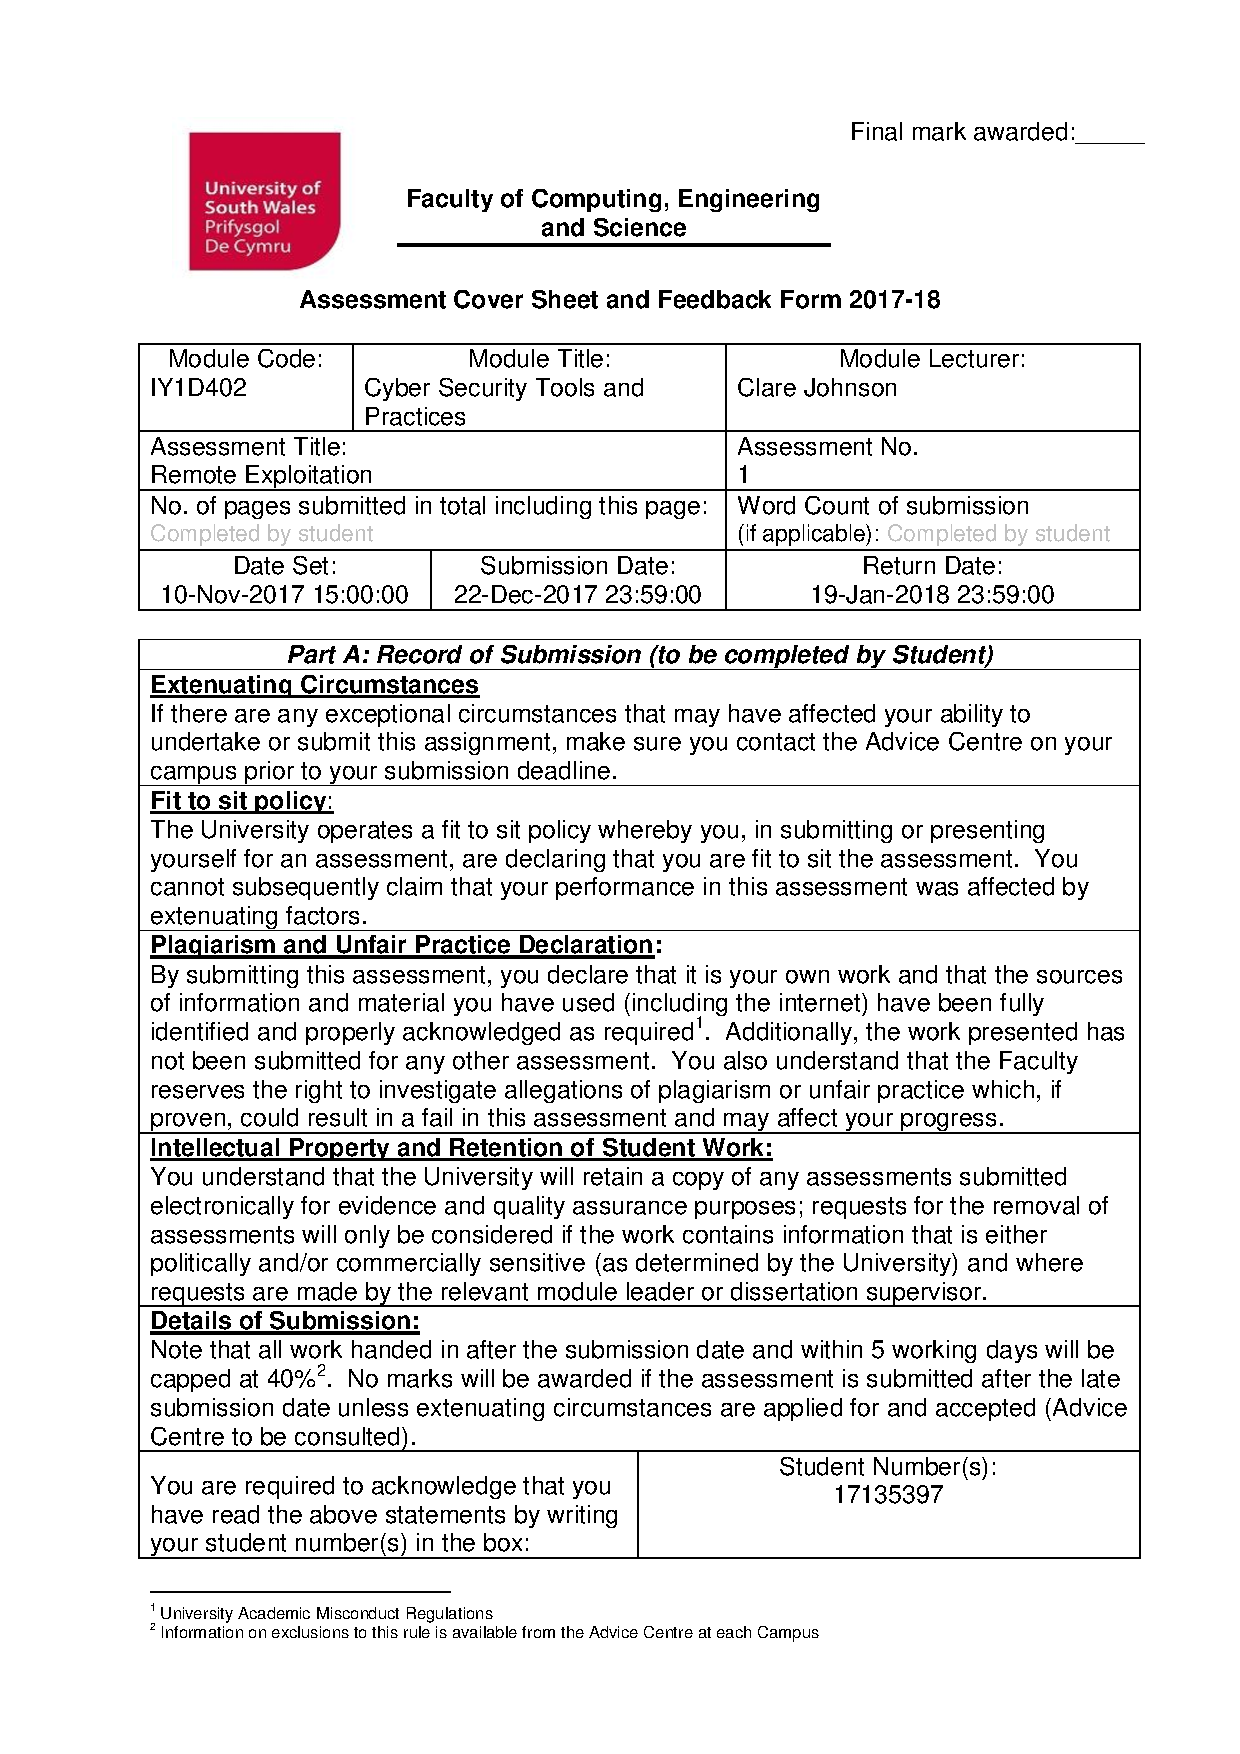
\includepdf[pages={1}]{assignmentbrief/IY1D402_CW1M_Cover_PRO_PROJECT1.pdf}
\tableofcontents
% -


% Pre-main configuration
% Increase the line spacing to 1.5x(=1.3) or 2x(=1.6)
% \linespread{1.0}
% \selectfont


\pagebreak
\section{Introduction}
For the first formal assessment of our IY1D402 \textit{(Cyber Security Tools and Practices)} we have been given a real-world scenario. We have been asked to, individually, conduct an investigation before writing a report that details the methodology that we followed during our investigation, presents our findings, discusses the capabilities of the tools we used, describes alternative methods that could have been used, and explains the nature of \textit{'insider threat'}. The target audience is a Senior Management Team and so, although it is a technical, this report will attempt to present technical aspects with enough explanation to make them understandable by those who are not technical specialists.

\subsection{Scenario}
I am the Senior Technical Officer at eCorp and have been asked by the Senior Management Team to investigate an employee -- Phillip Price -- who is suspected of exfiltrating Intellectual Property (IP) from the company.

To verify this suspicion, I have been asked to monitor Price's activities on the company's IT system, and have been given permission to use any appropriate methods in the course of this investigation. It has also been requested that I take suitable steps to conceal this monitoring from Price.

Upon completion of the investigation, I have been asked to write a report for the Senior Management Team that details exactly the steps that I took and explains my findings. I should also discuss the capabilities of the tools that I used and explain whether any alternative methods could have been used at various stages of the investigation.

Finally, to complete the report, I should explain the nature of \textit{'insider threat'} and its implications to an organisation while giving examples of where such threats have occurred in the past, discussing how the tools that I used impact on the organisation's security, and suggesting methods for improving our security in the future.


\pagebreak
\section{Preliminary Report}

\pagebreak
\section{Investigative Methodology}

\pagebreak
\section{Insider Threat}

\pagebreak
\section{Conclusion}


% Post-main configuration
% Increase the line spacing to 1x(=1.0), 1.5x(=1.3) or 2x(=1.6)
% \linespread{1.0}
% \selectfont


% BIBLIOGRAPHY/REFERENCES
\pagebreak
% nocited refs
\nocite{example:referenceid:here}

% Insert references section, left aligned
\begin{flushleft}
  \bibliography{references}
\end{flushleft}


% APPENDICES
\appendix

\pagebreak
\section{Appendix 1: screenshot deliverables}

\pagebreak
\section{Appendix 2: code deliverables}


\end{document}
